\section{Assignment Part B}
\label{sec:assignment_part_B}

In this section, we provide a brief overview of the requests associated with the second part of the assignment, along with a description of the approach taken to fulfill them.
Discussion of the results obtained is also included in the following sections.


\subsection{Request}
\label{subsec:request_part_B}

Given that in the previous section we have estimated the control commands sent to the robot during the original simulation, in this second part we are asked to evaluate the accuracy of such commands.



\subsection{Analysis}
\label{subsec:analysis_part_B}

In order to evaluate the accuracy of the control commands sent to the robot during the simulation, we need to rerun a simulation by our own, using the same world and the same robot model, and then compare both the trajectory and the velocities with the ones saved in the original \texttt{rosbag} file.

We recall that our working environment is setup so that \texttt{ROS1} is running in the \texttt{WSL2} (Windows Subsystem for Linux) environment, specifically in \texttt{Ubuntu 20.04}, while \texttt{MATLAB 2024a} is running in Windows 10.
Based on these considerations, we can run the simulation in at least three different ways:

\begin{itemize}
    \item Create a publisher script in \texttt{MATLAB} that sends the commands to \texttt{ROS1} running in \texttt{WSL2};
    \item Create a publisher in \texttt{Simulink} that sends the commands to \texttt{ROS1} running in \texttt{WSL2};
    \item Perform the analysis directly in \texttt{WSL2} using the native commands of \texttt{rosbag} to automatically replay the estimated commands.
\end{itemize}

At first, we tried to create a publisher script in \texttt{MATLAB} that was sending the commands over the bridged network, pacing the sender based on the original timing of the \texttt{/odom} topic.
However, we encountered some major issues with the timing of the commands, which were sent at almost unpredictable intervals, leading to a completely different behavior of the robot in the simulation.

In order to avoid or at least reduce the issues related to the timing of the commands, we decided to directly move to the third option, which is to perform the analysis directly in \texttt{WSL2} using the native commands of \texttt{rosbag} to automatically replay the estimated commands.
At first, the \texttt{/odom} topic has been ported to a new \texttt{rosbag} file using a simple \texttt{python} script, which is able to read the original \texttt{rosbag} file and write the \texttt{/odom} topic to a new \texttt{rosbag} file while also reshaping the data to match the type of the \texttt{/cmd\_vel} topic.
In particular, the following relationship table has been implemented:

\begin{table}[H]
    \centering
    \begin{tabular}{c|c}
        \textbf{/odom}            & \textbf{/cmd\_vel} \\
        \hline
        msg.Twist.Twist.Linear.X  & msg.Linear.X       \\
        msg.Twist.Twist.Angular.Z & msg.Angular.Z      \\
        \hline
    \end{tabular}
    \caption{Relationship between the \texttt{/odom} and \texttt{/cmd\_vel} topics.}
    \label{tab:rosbag_relationship}
\end{table}

Once the content of the \texttt{/odom} topic has been saved as \texttt{/cmd\_vel} topic in a new \texttt{rosbag} file, we can use the \texttt{rosbag play} command to replay the commands in the simulation.

In Figure \ref{fig:trajectory_comparison} we can see the comparison of the trajectories performed by the original simulation and the one performed by the replayed commands.

\begin{figure}[H]
    \centering
    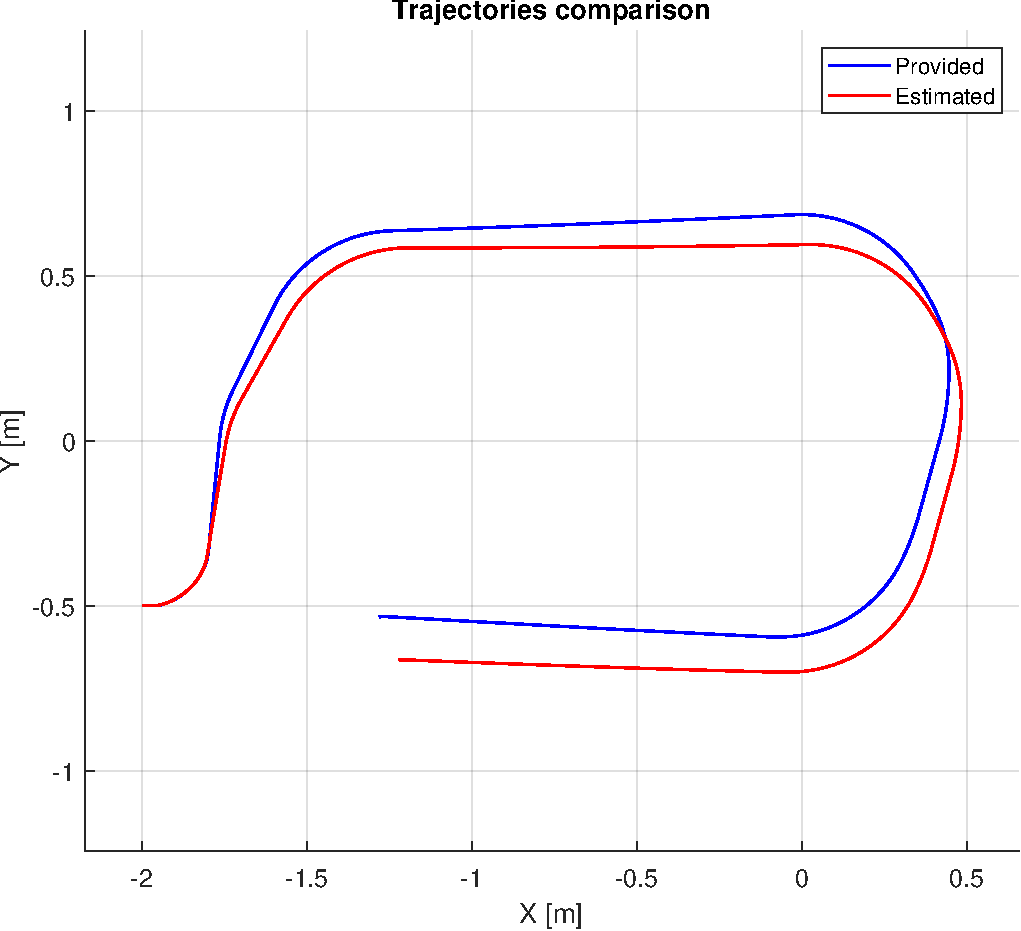
\includegraphics[width=0.8\textwidth]{./img/MATLAB/trajectories_comparison.pdf}
    \caption{Comparison of the trajectories performed by the original simulation and the one performed by the replayed commands.}
    \label{fig:trajectory_comparison}
\end{figure}

One can clearly see that the two trajectories are not completely overlapping.

Looking at the values of the actual velocities of the robot during the simulation, we can see a minor discrepancy between the original simulation and the one performed by the replayed commands, similarly to the behaviour observer for the trajectories.
Figure \ref{fig:velocity_comparison} shows the comparison of the velocities performed by the original simulation and the one performed by the replayed commands.

\begin{figure}[H]
    \centering
    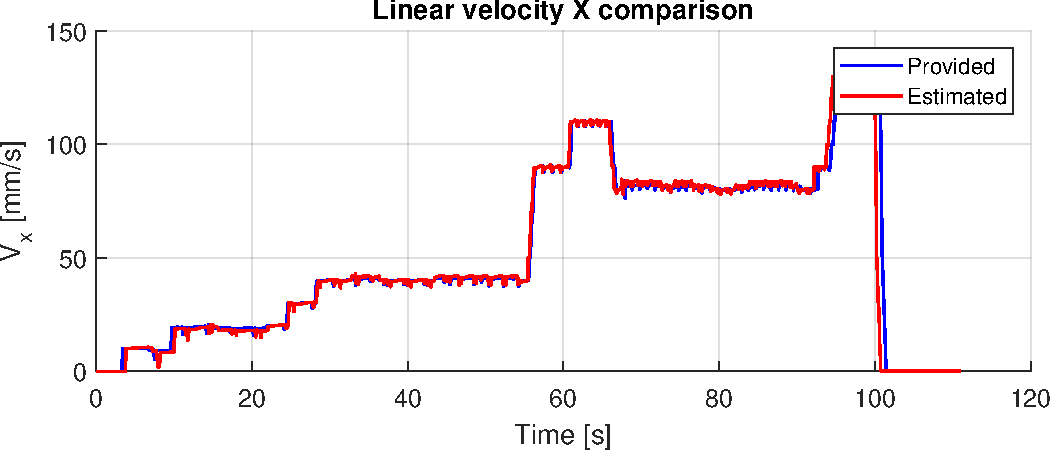
\includegraphics[width=0.8\textwidth]{./img/MATLAB/linear_velocity_comparison.pdf}

    \vspace{10pt}

    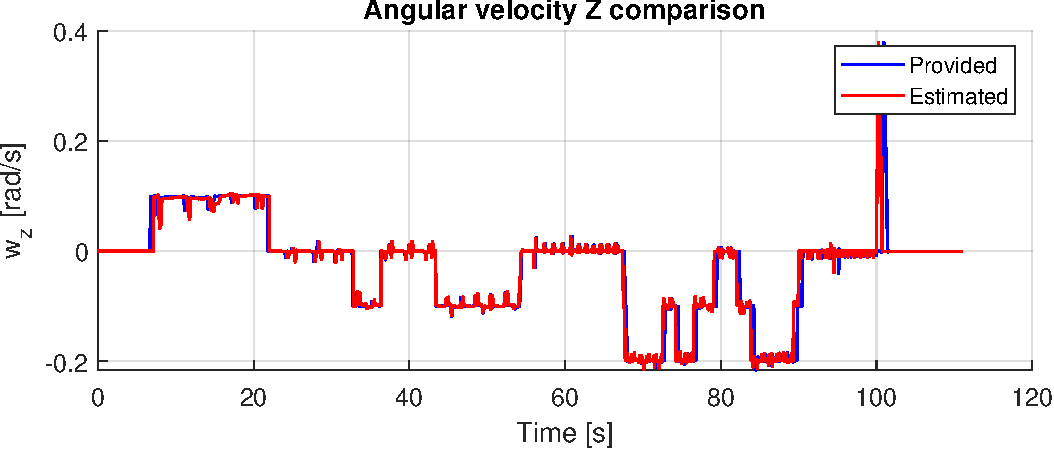
\includegraphics[width=0.8\textwidth]{./img/MATLAB/angular_velocity_comparison.pdf}
    \caption{Comparison of the velocities performed by the original simulation and the one performed by the replayed commands.}
    \label{fig:velocity_comparison}
\end{figure}

Again, some minor issues related to timing can be observed.
For some reason that the author is not able to determine, the \texttt{rosbag play} command is not able to replay the commands at the exact same pace as the original simulation, leading to a slight shift in the velocities.

What is also interesting to notice, are the juggling of the velocities along the whole simulation.
These are, in fact, not desired behaviors and most probably caused by the simulated environment itself.